\documentclass[11pt,a4paper]{article}
\usepackage{fontspec}
\setmainfont{TeX Gyre Pagella}
\newfontfamily\headfont{Inter}[UprightFont=*-ExtraBold,BoldFont=*-ExtraBold,Extension=.otf,Path=/usr/share/fonts/opentype/inter/]
\usepackage[a4paper,margin=2.3cm]{geometry}
\usepackage{graphicx,booktabs,float,caption,array,xcolor,longtable}
\usepackage{xurl}
\usepackage[hidelinks]{hyperref}
\usepackage{titlesec}
\usepackage[round]{natbib}
\usepackage{setspace}
\setstretch{1.05}
\renewcommand{\topfraction}{0.9}
\renewcommand{\bottomfraction}{0.8}
\renewcommand{\textfraction}{0.1}
\renewcommand{\floatpagefraction}{0.75}
\setlength{\parindent}{0pt}
\setlength{\parskip}{0.55em}
\titleformat{\section}{\headfont\Large}{\thesection}{0.8em}{}
\titleformat{\subsection}{\headfont\large}{\thesubsection}{0.8em}{}
\captionsetup{font=small,labelfont=bf}
\urlstyle{same}
\hypersetup{pdftitle={Shadows of the Giants},pdfauthor={Tristan Hotham}}

\begin{document}
\begin{center}
{\Large\bfseries Shadows of the Giants\par}
\vspace{0.4em}
{\large Winter sun at street level and the shadows of tall buildings in eight UK city centres\par}
\vspace{1.2em}
{\large Tristan Hotham\par}
\vspace{0.3em}
{\small Independent researcher\\
ORCID: 0000-0003-4931-9349\\
DOI: https://doi.org/10.5281/zenodo.24075303\par}
\vspace{0.8em}
2026
\end{center}

\begin{quote}
\small
\begin{center}\textbf{Abstract}\end{center}
Tall buildings cast long shadows when the sun is low. I model direct sunlight at street level on 21 December, 20 March and 21 June in eight UK city centres (central London, Canary Wharf, Manchester, Birmingham, Leeds, Liverpool, Glasgow and Edinburgh) from OpenStreetMap building heights served as OpenFreeMap vector tiles, on a 5 m grid with the terrain beneath, with the sun traced every ten minutes. Comparing each centre as built with the same centre without its towers (building parts of 50 m or more) and without any buildings separates the shadow of the towers from that of the ordinary city. At noon on the winter solstice a shadow is 3.7 times the height of what casts it in London and 5.3 times in Edinburgh; the Shard (310 m in OpenStreetMap) throws a noon shadow of 1,146 m. On the average square metre of open ground, direct sun on 21 December ranges from 2.1 hours (Edinburgh) to 3.4 hours (Leeds), against 6.8 to 7.7 hours with a flat horizon. Most of the loss is due to ordinary buildings: towers take 0.18 hours in central London but 0.76 hours at Canary Wharf, where 25.9\% of open ground loses an hour or more to them, and 0.48 hours in Manchester. Building heights are incomplete: 41.4\% to 73.7\% of footprint area carries neither a height nor a storey count and is drawn 5 m high, so the shadows of ordinary buildings are underestimated.

\textbf{Keywords:} urban shadow; sunlight; tall buildings; OpenStreetMap; building heights; winter solstice; street canyons; United Kingdom
\end{quote}

\section{Introduction}
Sunlight in streets and public spaces has long been a planning concern, and in the United Kingdom guidance on daylight and sunlight in new development is set out by the Building Research Establishment \citep{bre2022}. Most assessments model one scheme in detail. This study asks a broader, comparative question with open data: across the centres of eight large UK cities, how much winter sun reaches street level, and how much of what is lost is due to the towers rather than to the ordinary dense city? It also measures how complete open building heights are, since every answer depends on them.

\section{Data}
\textbf{Buildings, streets and open spaces.} OpenFreeMap \citep{openfreemap} serves OpenStreetMap \citep{osm} in the OpenMapTiles schema; I used the zoom-14 tiles of release 20261101\_080013\_pt. The building layer gives each building part a \texttt{render\_height}: the OpenStreetMap height where tagged, otherwise the number of storeys times 3.66 m (rounded up), otherwise 5 m. Features in the tile are merged by height, so they cannot be counted as buildings; completeness is measured by footprint area (Table~\ref{tab:cities}, Figure~\ref{fig:heights}). Named streets come from the \texttt{transportation\_name} layer (roads, not footpaths), and open spaces from the \texttt{landcover} (park, garden, recreation ground, village green, common) and \texttt{park} layers, named from park and garden points of interest inside them.

\textbf{Terrain.} The ground beneath each centre is from the AWS Terrain Tiles at zoom 10 (about 90 m), interpolated bilinearly.

\textbf{Centres.} Each centre is a box of about 3 by 2 to 3 km (central London 8.3 by 5.8 km, from Westminster and Vauxhall to the City and the Southbank), on a 5 m grid in a transverse Mercator projection centred on it so that grid north is true north, with a margin of 1.2 km in which buildings are included so that they can cast shadows into the box.

\section{Method}
\textbf{Sun.} Solar position follows the NOAA general solar position equations, with the declination and equation of time from the Fourier series of \citet{spencer1971} and refraction after \citet{saemundsson1986}, at the centre of each box, every ten minutes from sunrise to sunset on 21 December, 20 March and 21 June 2026.

\textbf{Shadows.} For each sun position the surface (ground plus building height) is swept along lines parallel to the sun's azimuth, one cell at a time along the dominant axis so that every cell is visited once; along each line the height of the shadow line falls by the step length times the tangent of the solar altitude and is raised by any surface above it, and a cell is in shadow when the shadow line is above the surface there. A test block confirms the direction and the length $h/\tan\alpha$ of its shadow. Three surfaces are swept: terrain only; terrain with building parts under 50 m (the city without its towers); and terrain with all buildings. Open ground is every cell with no building and no water inside the box. A tower is a set of touching building parts of 50 m or more whose merged footprint is at least 300 m$^2$; thinner ones (spires, chimneys, masts) are counted separately. The surface without towers drops every part of 50 m or more, thin ones included; keeping the thin parts changes the hours taken by towers by less than 0.01 h in every centre. Hours of direct sun per cell are the number of ten-minute steps in sun. A street's value is the average over cells within 4 m of its centre line that are open ground.

\section{Results}
\subsection{Long winter shadows}
On 21 December the noon sun reaches 15.1\textdegree{} in London and 10.7\textdegree{} in Edinburgh, so a shadow at noon is 3.7 and 5.3 times the height respectively (Figure~\ref{fig:length}; 3.70 and 5.28 with refraction, 3.71 and 5.32 without it); a 300 m tower in London would cast a noon shadow of 1,110 m. The tallest tower in the data, the Shard at 310 m, casts 1,146 m at noon on the solstice, 1,649 m two hours before noon and 1,642 m two hours after, 395 m at noon at the equinox and 165 m at midsummer. Table~\ref{tab:towers} lists the towers with the longest noon shadows in December.

\begin{figure}[tbp]\centering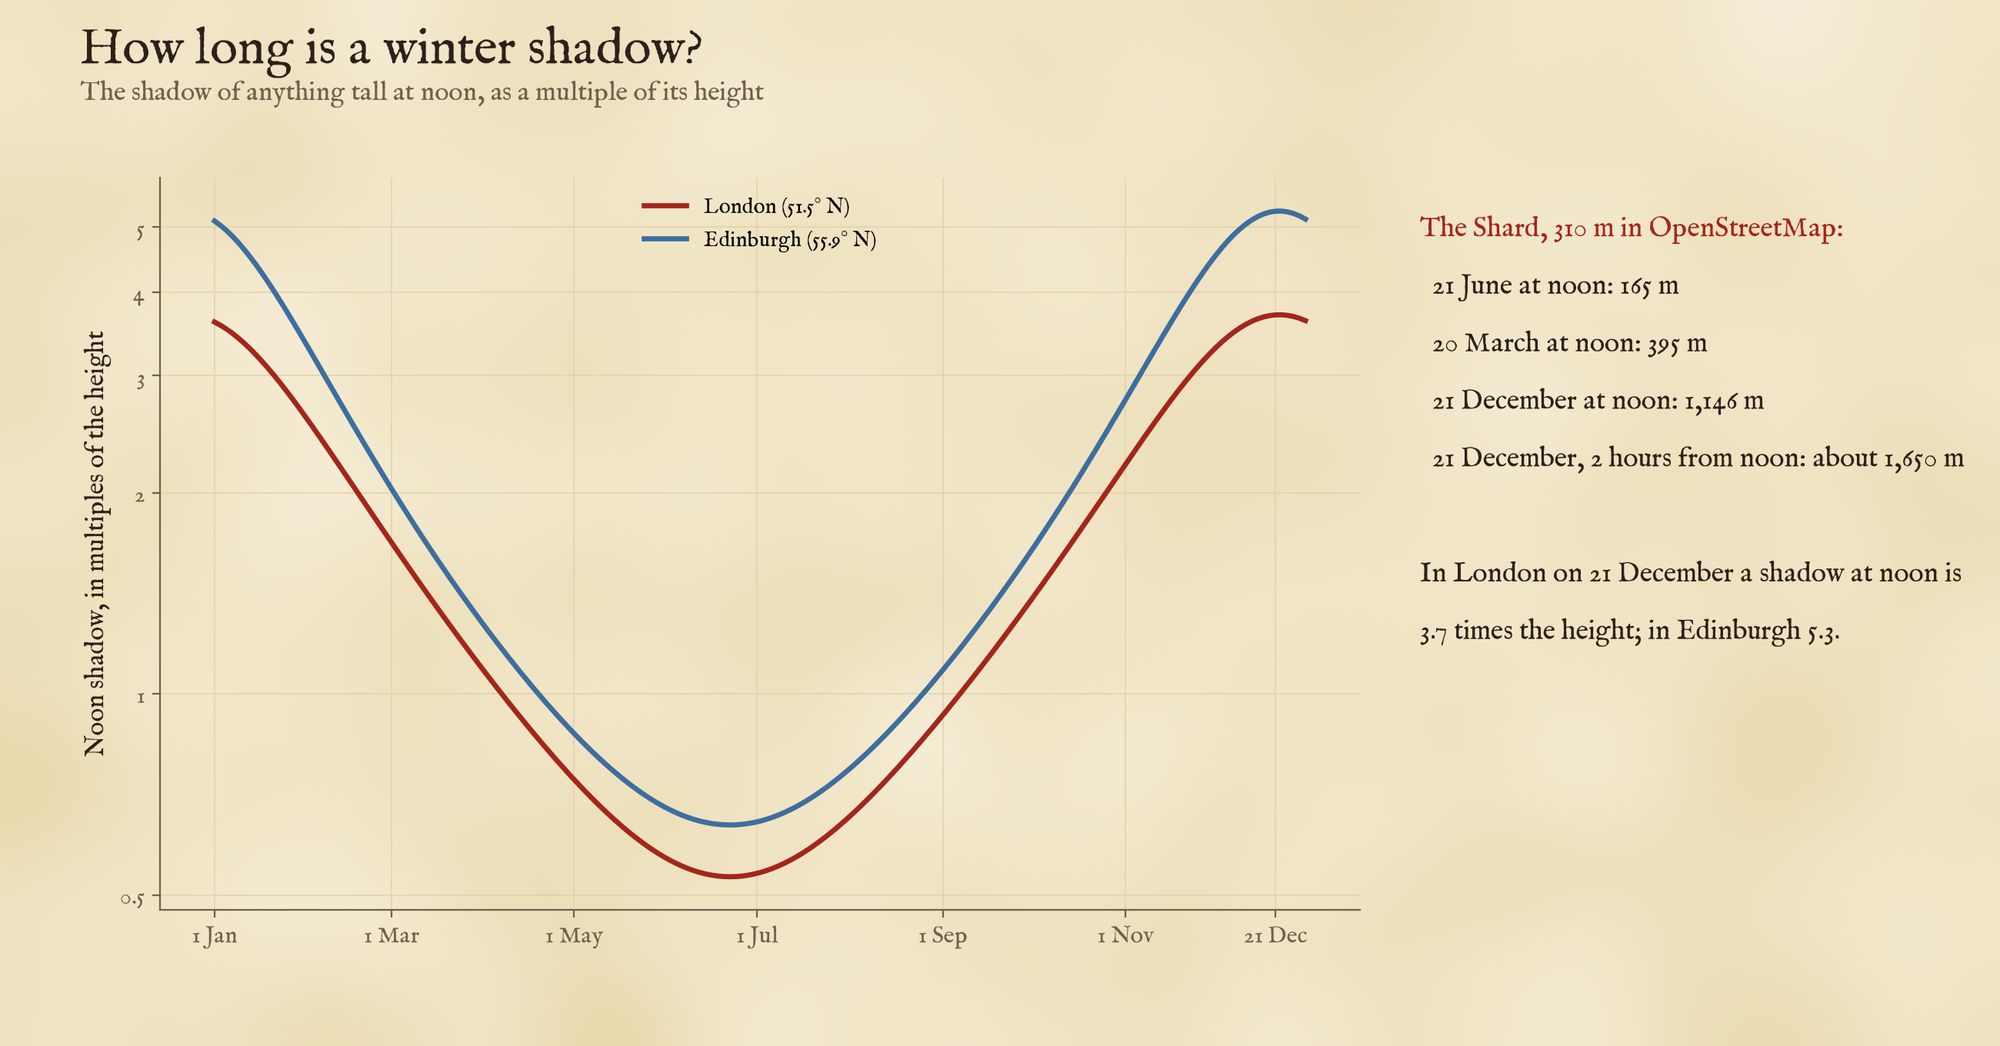
\includegraphics[width=\textwidth]{f_length.png}
\caption{The noon shadow as a multiple of the height through the year in London and Edinburgh.}\label{fig:length}\end{figure}

\begin{table}[tbp]\centering\small\caption{Towers with the longest noon shadows on 21 December (flat ground), with the shadow two hours either side of noon. Heights are OpenStreetMap render heights; the first is the Shard.}\label{tab:towers}\begin{tabular}{lrlrr}\toprule Centre & Height (m) & Position & Noon (m) & $\pm$2 h (m)\\\midrule
Central London & 310 & 51.5044, -0.0864 & 1,146 & 1,645\\
Central London & 278 & 51.5142, -0.0832 & 1,027 & 1,476\\
Canary Wharf & 275 & 51.5027, -0.0255 & 1,016 & 1,460\\
Canary Wharf & 249 & 51.5010, -0.0173 & 920 & 1,322\\
Central London & 242 & 51.4843, -0.1272 & 894 & 1,285\\
Canary Wharf & 235 & 51.5049, -0.0195 & 869 & 1,248\\
Manchester & 201 & 53.4719, -2.2516 & 859 & 1,279\\
Central London & 231 & 51.5162, -0.0809 & 854 & 1,226\\
Central London & 225 & 51.5139, -0.0823 & 832 & 1,194\\
Manchester & 191 & 53.4721, -2.2560 & 816 & 1,215\\
\bottomrule\end{tabular}\end{table}

\subsection{Sun at street level}
Table~\ref{tab:cities} and Figure~\ref{fig:compare} give the average hours of direct sun on open ground on 21 December in each centre, as built, without the towers, without any buildings, and against a flat horizon. In every centre the ordinary buildings take most of the winter sun: in central London the average square metre of open ground gets 2.84 hours of a possible 7.67, and 21.9\% gets none. The towers' own share is largest at Canary Wharf (0.76 hours on average, and an hour or more for 25.9\% of open ground; Figure~\ref{fig:canary}) and in Manchester (0.48 hours). Edinburgh, with 1 tower in its centre, is nonetheless the darkest (32.6\% of open ground without direct sun). Its terrain takes about an hour of a 7.0 hour day on average, more than in any other centre, but terrain alone leaves only 0.7\% of open ground without sun. The all-day shade is cast by ordinary buildings under a noon sun 10.7\textdegree{} up: swept on flat ground, the buildings alone leave 28.8\% without sun, and the buildings on the Old Town ridge, above the valleys either side, add the rest.

\begin{table}[tbp]\centering\footnotesize\caption{Eight centres on 21 December: towers (50 m or more, footprint 300 m$^2$ or more), share of building footprint at the 5 m default (\%), and average hours of direct sun on open ground with a flat horizon, with terrain only, without towers and as built; share of open ground with no direct sun (\%); hours taken by towers; share of open ground losing an hour or more to towers (\%).}\label{tab:cities}\begin{tabular}{lrrrrrrrrr}\toprule Centre & Towers & Default & Flat & Terrain & No towers & As built & No sun & Towers take & $\ge$1 h\\\midrule
Central London & 316 & 47 & 7.67 & 7.64 & 3.02 & 2.84 & 21.9 & 0.18 & 5.6\\
Canary Wharf & 107 & 41 & 7.67 & 7.64 & 3.36 & 2.60 & 20.0 & 0.76 & 25.9\\
Manchester & 103 & 47 & 7.50 & 7.26 & 3.08 & 2.60 & 19.2 & 0.48 & 19.2\\
Birmingham & 63 & 62 & 7.50 & 7.27 & 3.19 & 2.91 & 19.0 & 0.28 & 9.8\\
Leeds & 43 & 62 & 7.33 & 7.14 & 3.76 & 3.44 & 12.8 & 0.32 & 11.9\\
Liverpool & 28 & 74 & 7.33 & 7.14 & 3.49 & 3.23 & 13.8 & 0.27 & 8.6\\
Glasgow & 19 & 64 & 6.83 & 6.76 & 3.10 & 2.97 & 20.0 & 0.13 & 4.1\\
Edinburgh & 1 & 53 & 7.00 & 5.96 & 2.12 & 2.11 & 32.6 & 0.01 & 0.0\\
\bottomrule\end{tabular}\end{table}

\begin{figure}[tbp]\centering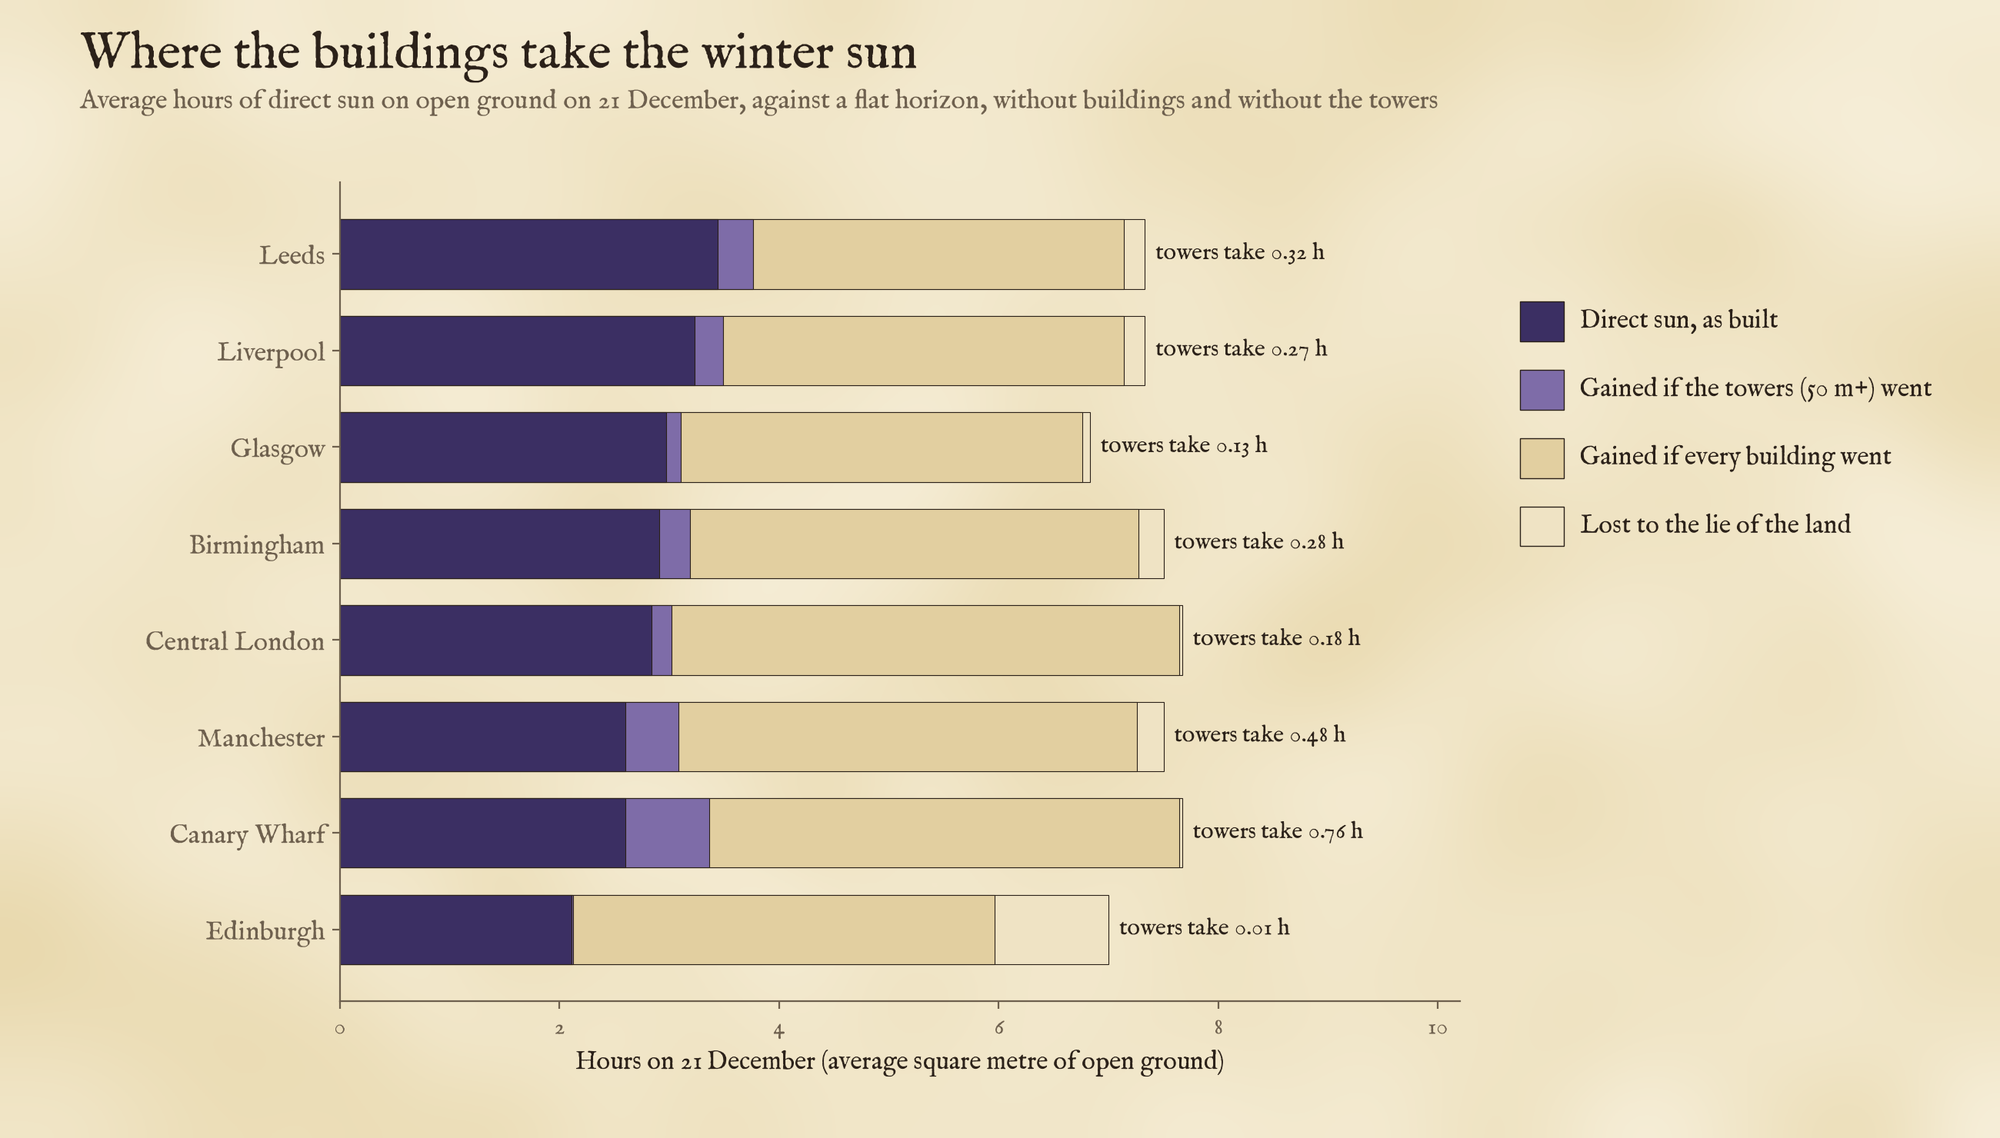
\includegraphics[width=\textwidth]{f_compare.png}
\caption{Average hours of direct sun on open ground on 21 December.}\label{fig:compare}\end{figure}

\begin{figure}[tbp]\centering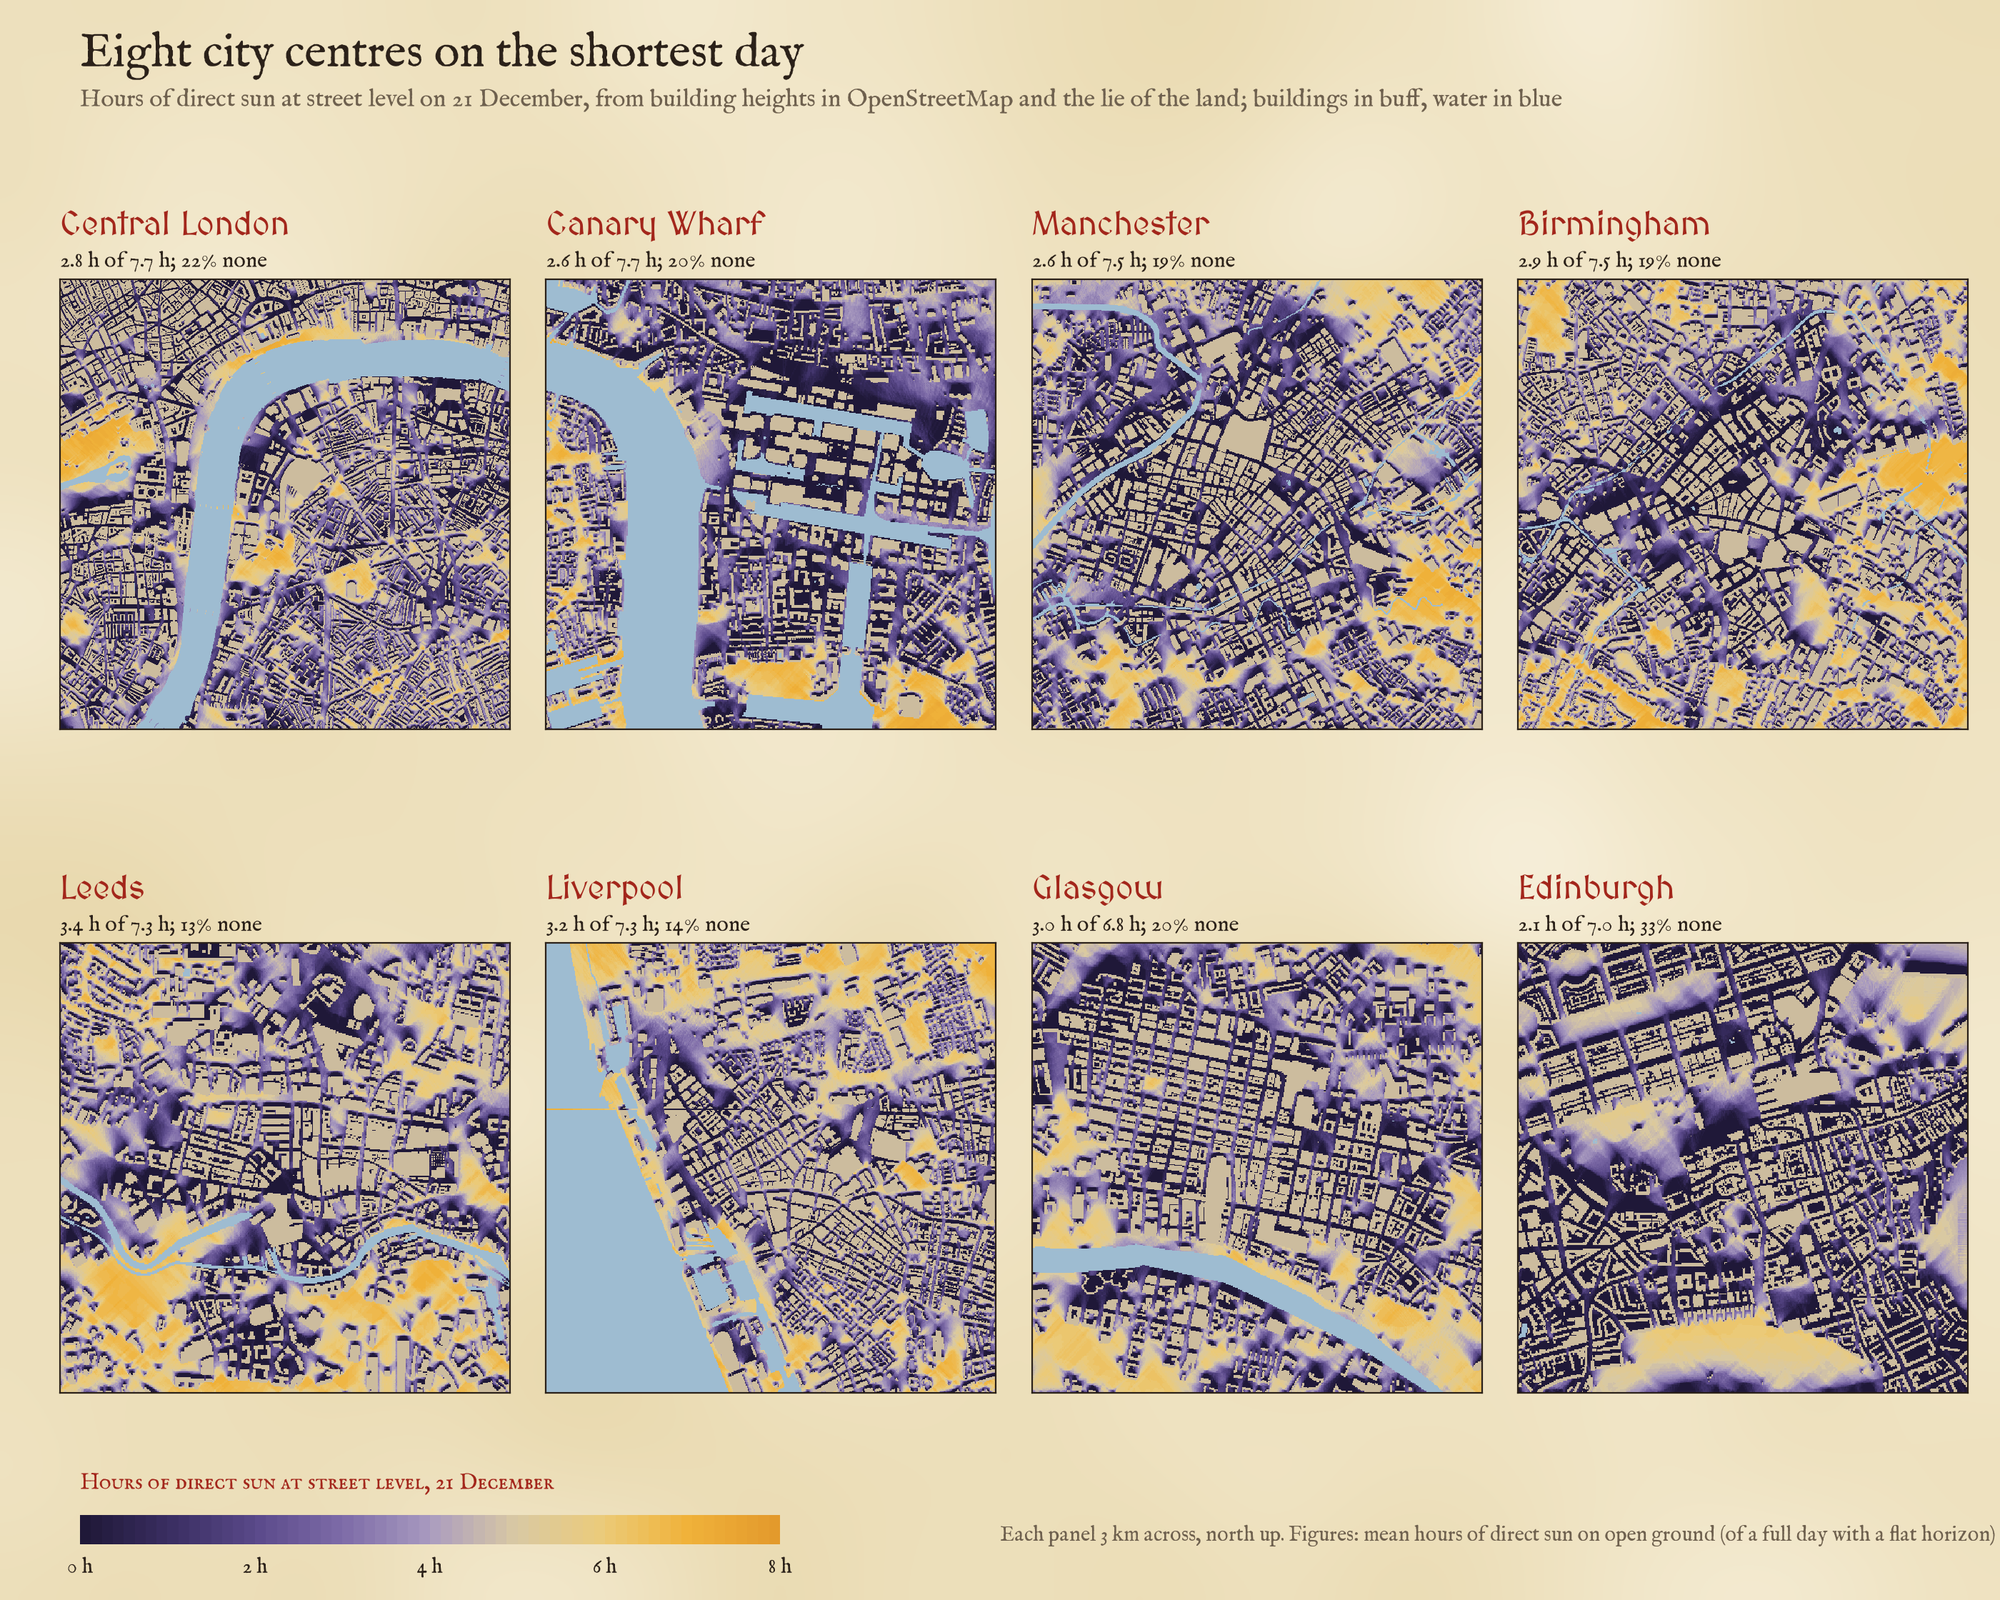
\includegraphics[width=\textwidth]{f_cities.png}
\caption{Hours of direct sun at street level on 21 December, central 3 km of each centre.}\label{fig:cities}\end{figure}

\begin{figure}[tbp]\centering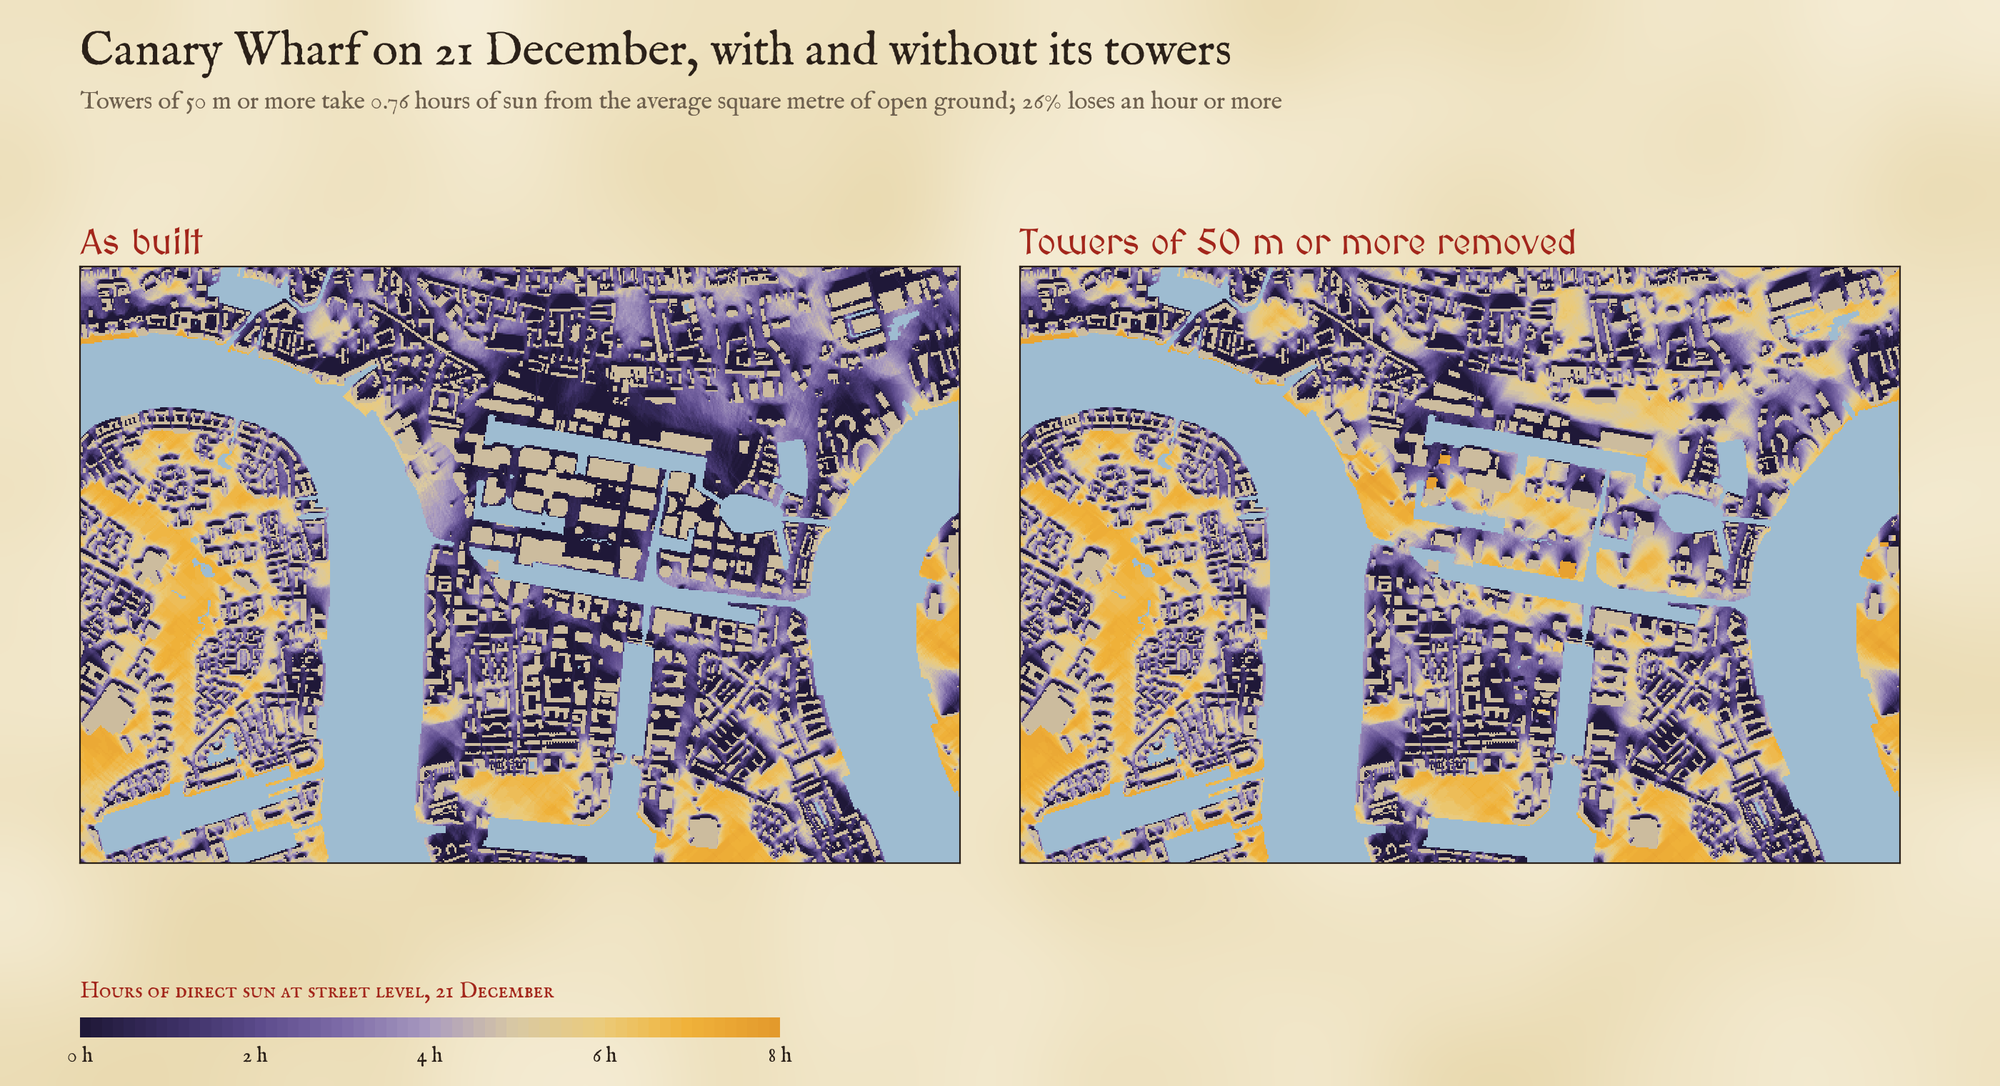
\includegraphics[width=\textwidth]{f_canary.png}
\caption{Canary Wharf on 21 December as built and with the towers removed.}\label{fig:canary}\end{figure}

\begin{figure}[tbp]\centering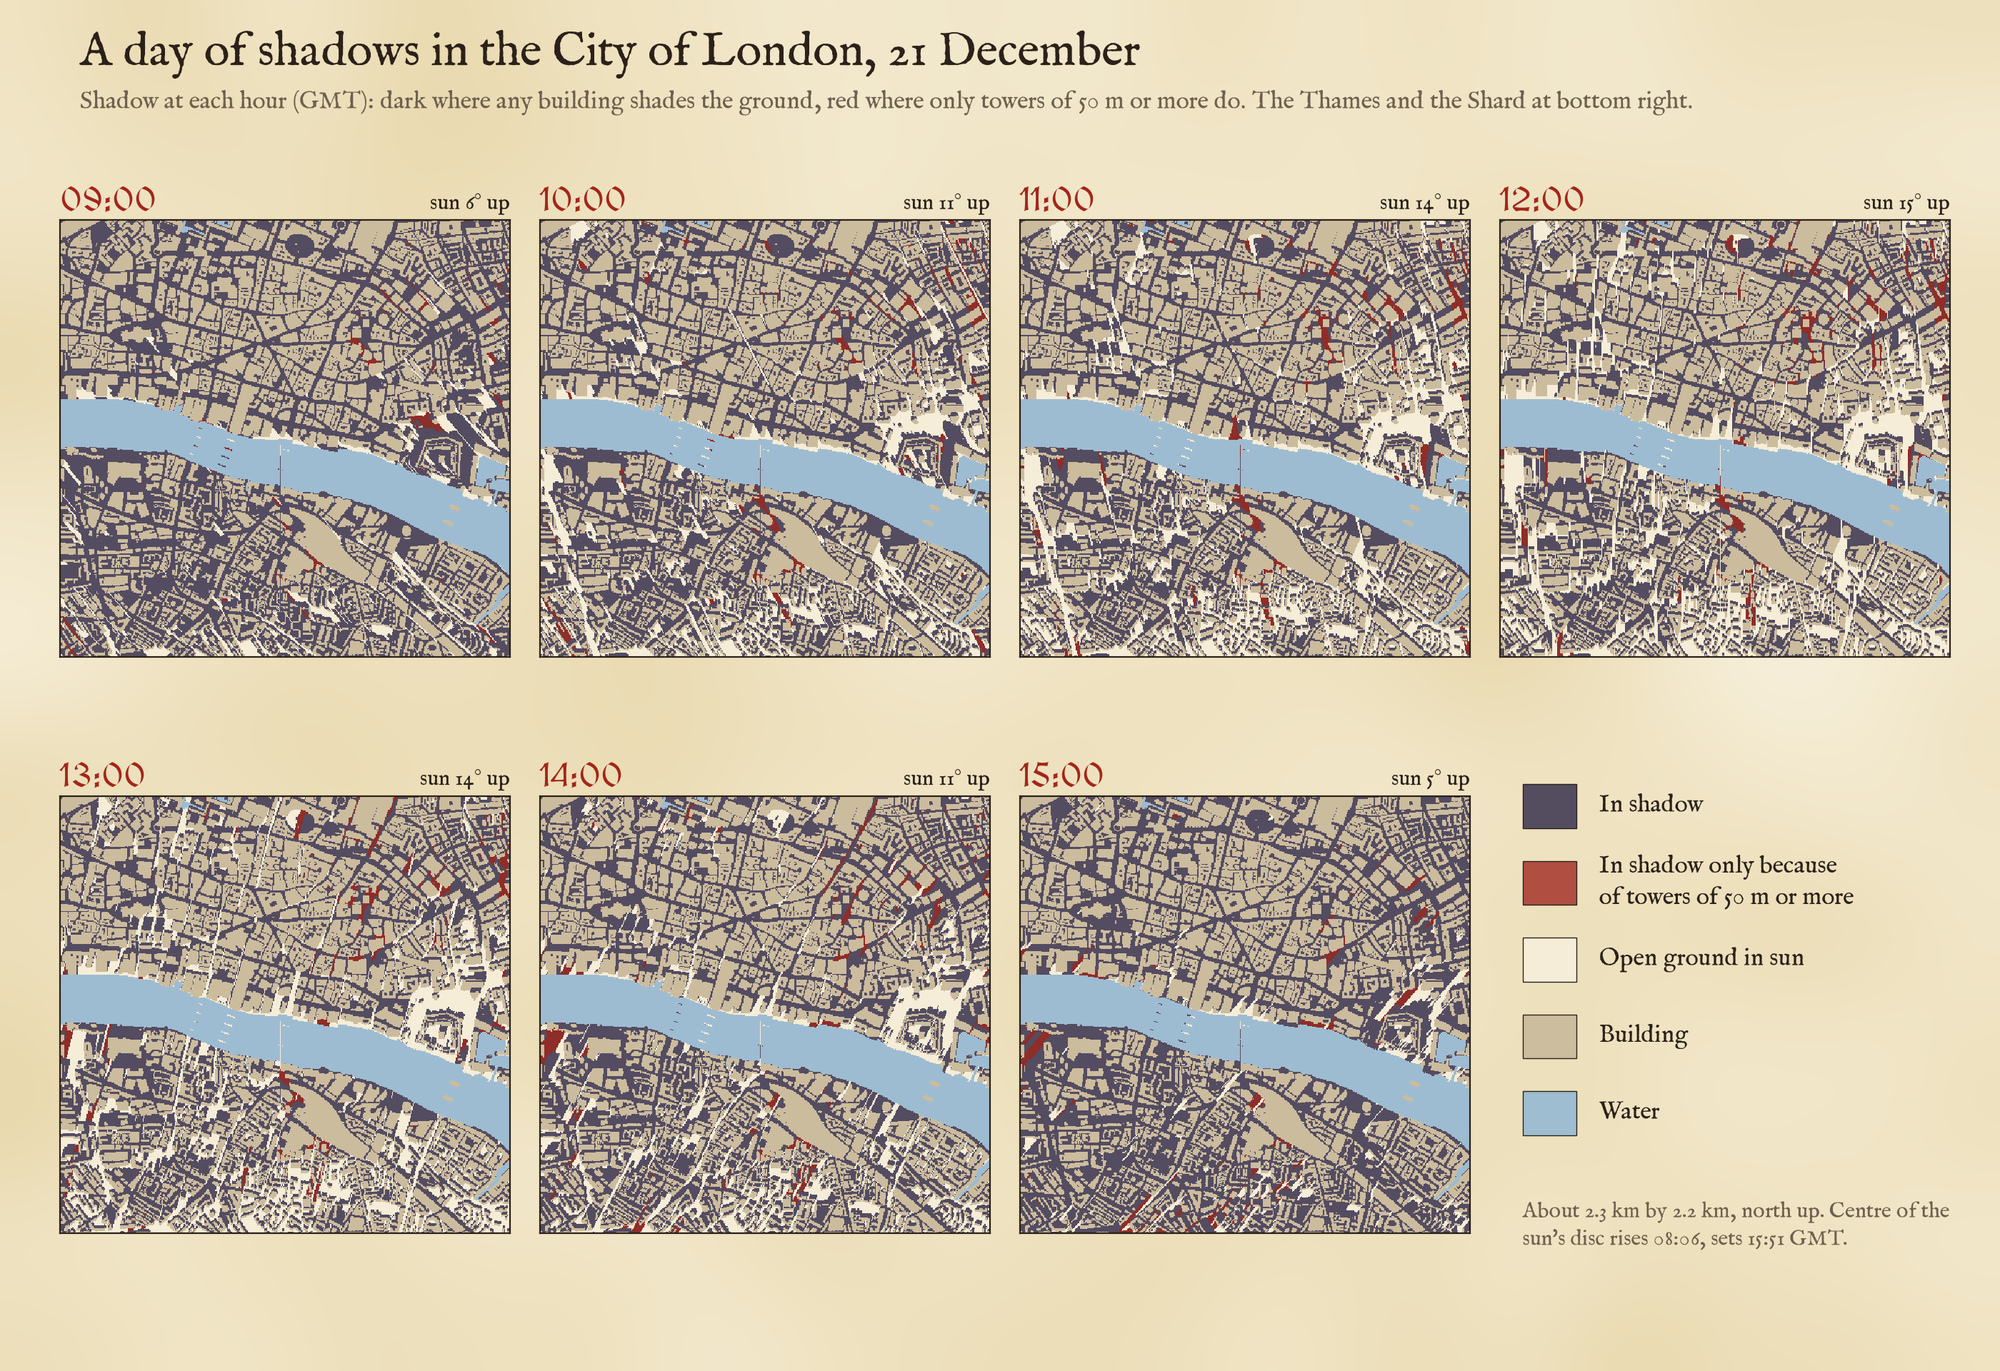
\includegraphics[width=\textwidth]{f_day.png}
\caption{Shadows hour by hour on 21 December in the City of London and the Southbank.}\label{fig:day}\end{figure}

\subsection{The most overshadowed streets and squares}
Of 3,469 named streets with at least 150 m inside the boxes, 1,094 average less than an hour of direct sun on 21 December and 209 lose an hour or more to towers. The largest losses to towers are at Canary Wharf, and in central London around Battersea Power Station and the new towers beside it, on the Marylebone Flyover, and at Elephant and Castle and Vauxhall (Table~\ref{tab:streets}, Figure~\ref{fig:streets}).

\begin{table}[tbp]\centering\small\caption{Streets (above) and open spaces (below) losing most direct sun to towers on 21 December: average hours as built, without towers and without buildings.}\label{tab:streets}\begin{tabular}{llrrr}\toprule Name & Centre & As built & No towers & No buildings\\\midrule
South Colonnade & Canary Wharf & 0.19 & 5.96 & 7.64\\
Circus Road South & Central London & 0.59 & 6.36 & 7.67\\
Water Street & Canary Wharf & 0.17 & 4.54 & 7.67\\
Castor Lane & Canary Wharf & 0.40 & 4.76 & 7.50\\
Canada Square & Canary Wharf & 0.03 & 4.13 & 7.52\\
Charter Street & Canary Wharf & 0.47 & 4.25 & 7.67\\
Bank Street & Canary Wharf & 0.26 & 3.94 & 7.67\\
Clove Crescent & Canary Wharf & 1.06 & 4.48 & 7.67\\
West Street & Leeds & 3.17 & 6.28 & 7.31\\
Sandford Street & Leeds & 1.18 & 4.26 & 7.29\\
\midrule
Canada Square Park & Canary Wharf & 0.00 & 5.55 & 7.50\\
Swedenborg Gardens & Central London & 0.59 & 4.51 & 7.67\\
Compton Gardens & Canary Wharf & 2.39 & 6.08 & 7.67\\
Jubilee Park & Canary Wharf & 0.12 & 3.74 & 7.67\\
Harbord Square Park & Canary Wharf & 0.64 & 3.37 & 7.67\\
\bottomrule\end{tabular}\end{table}

\begin{figure}[tbp]\centering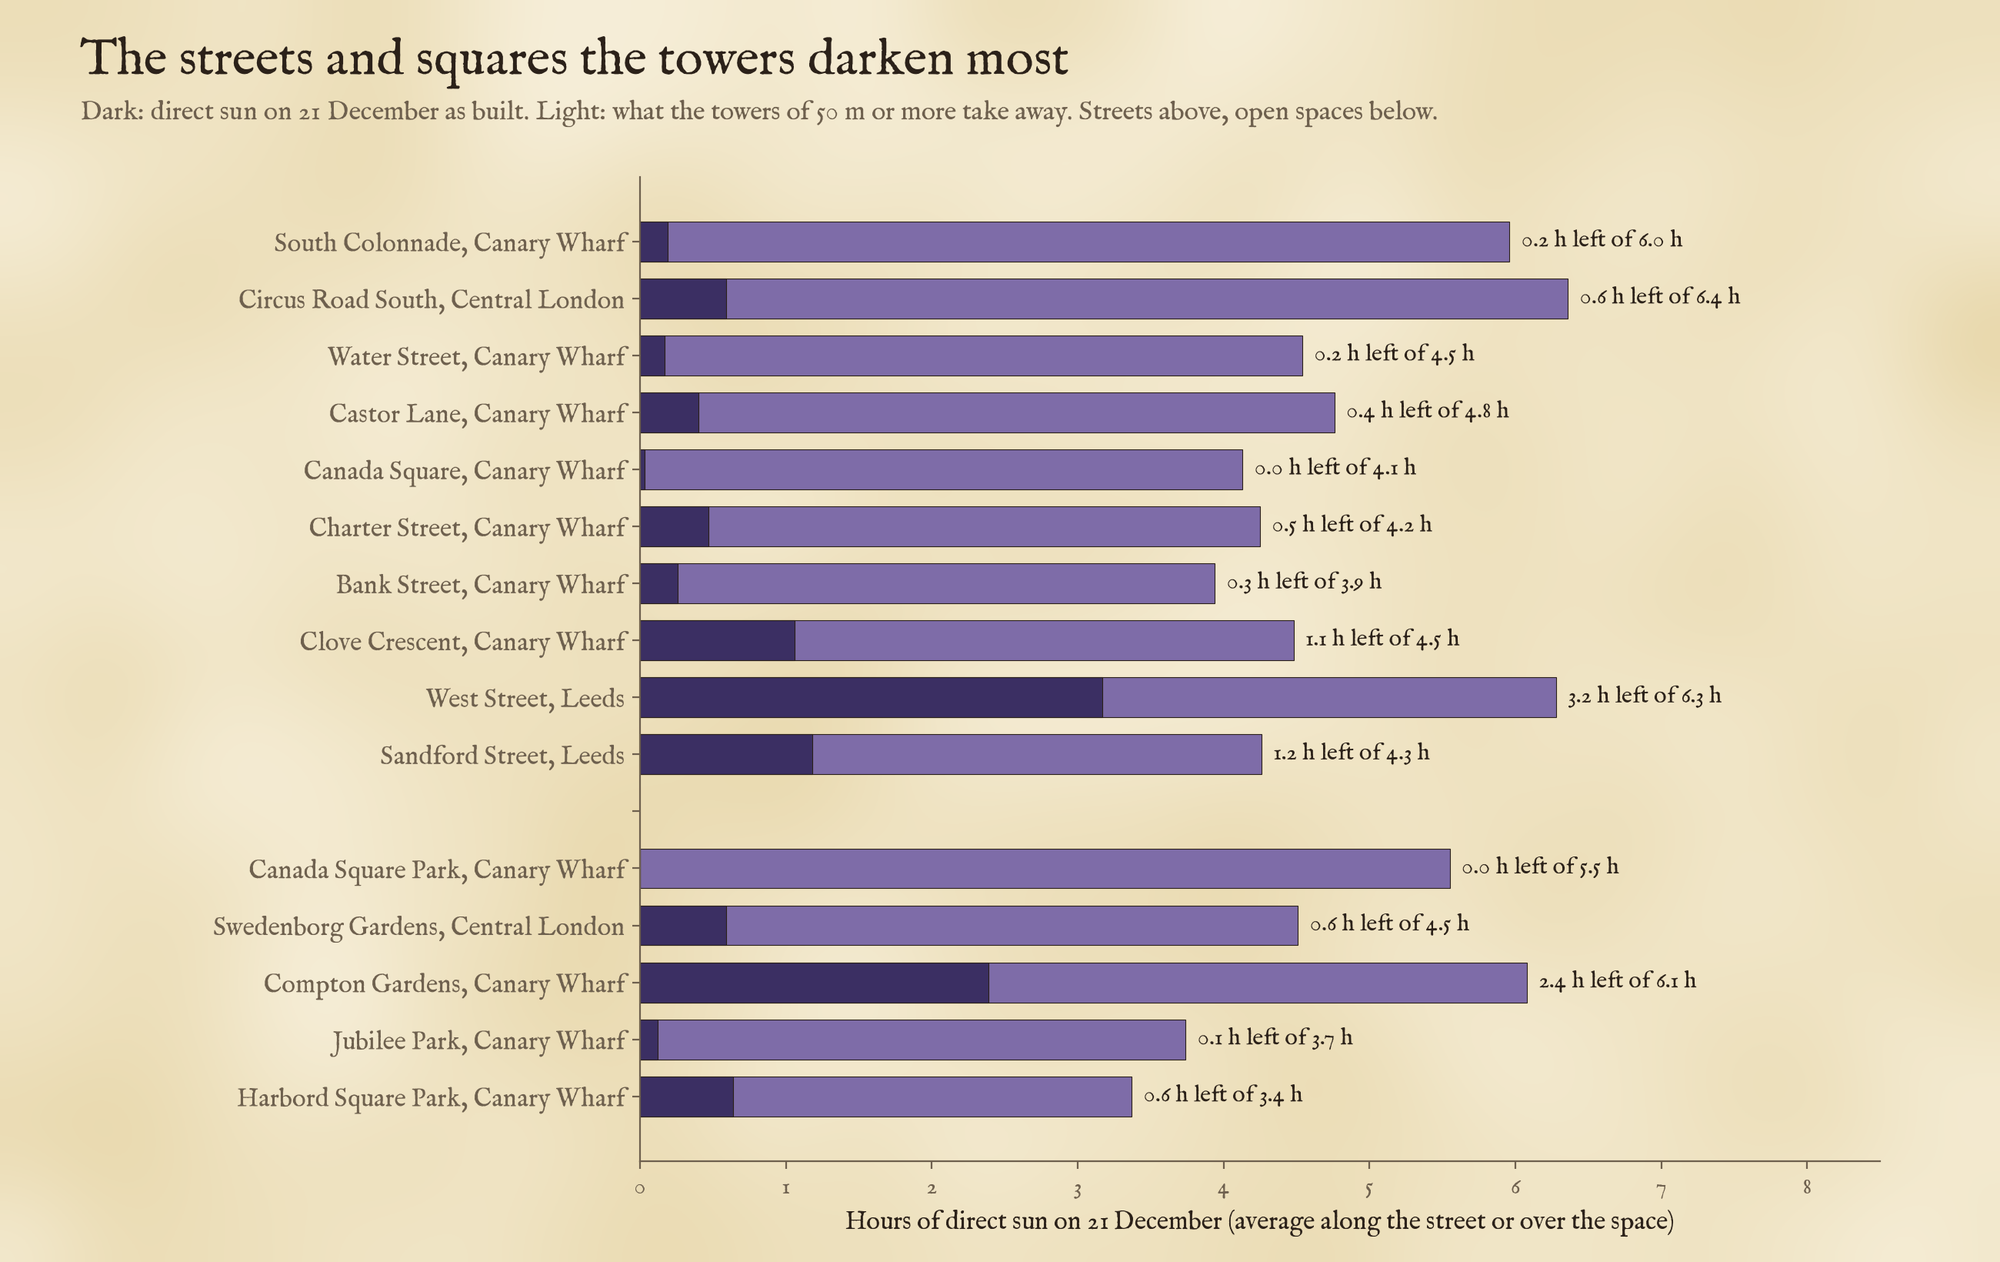
\includegraphics[width=\textwidth]{f_streets.png}
\caption{The streets and open spaces that lose most winter sun to towers.}\label{fig:streets}\end{figure}

\begin{figure}[tbp]\centering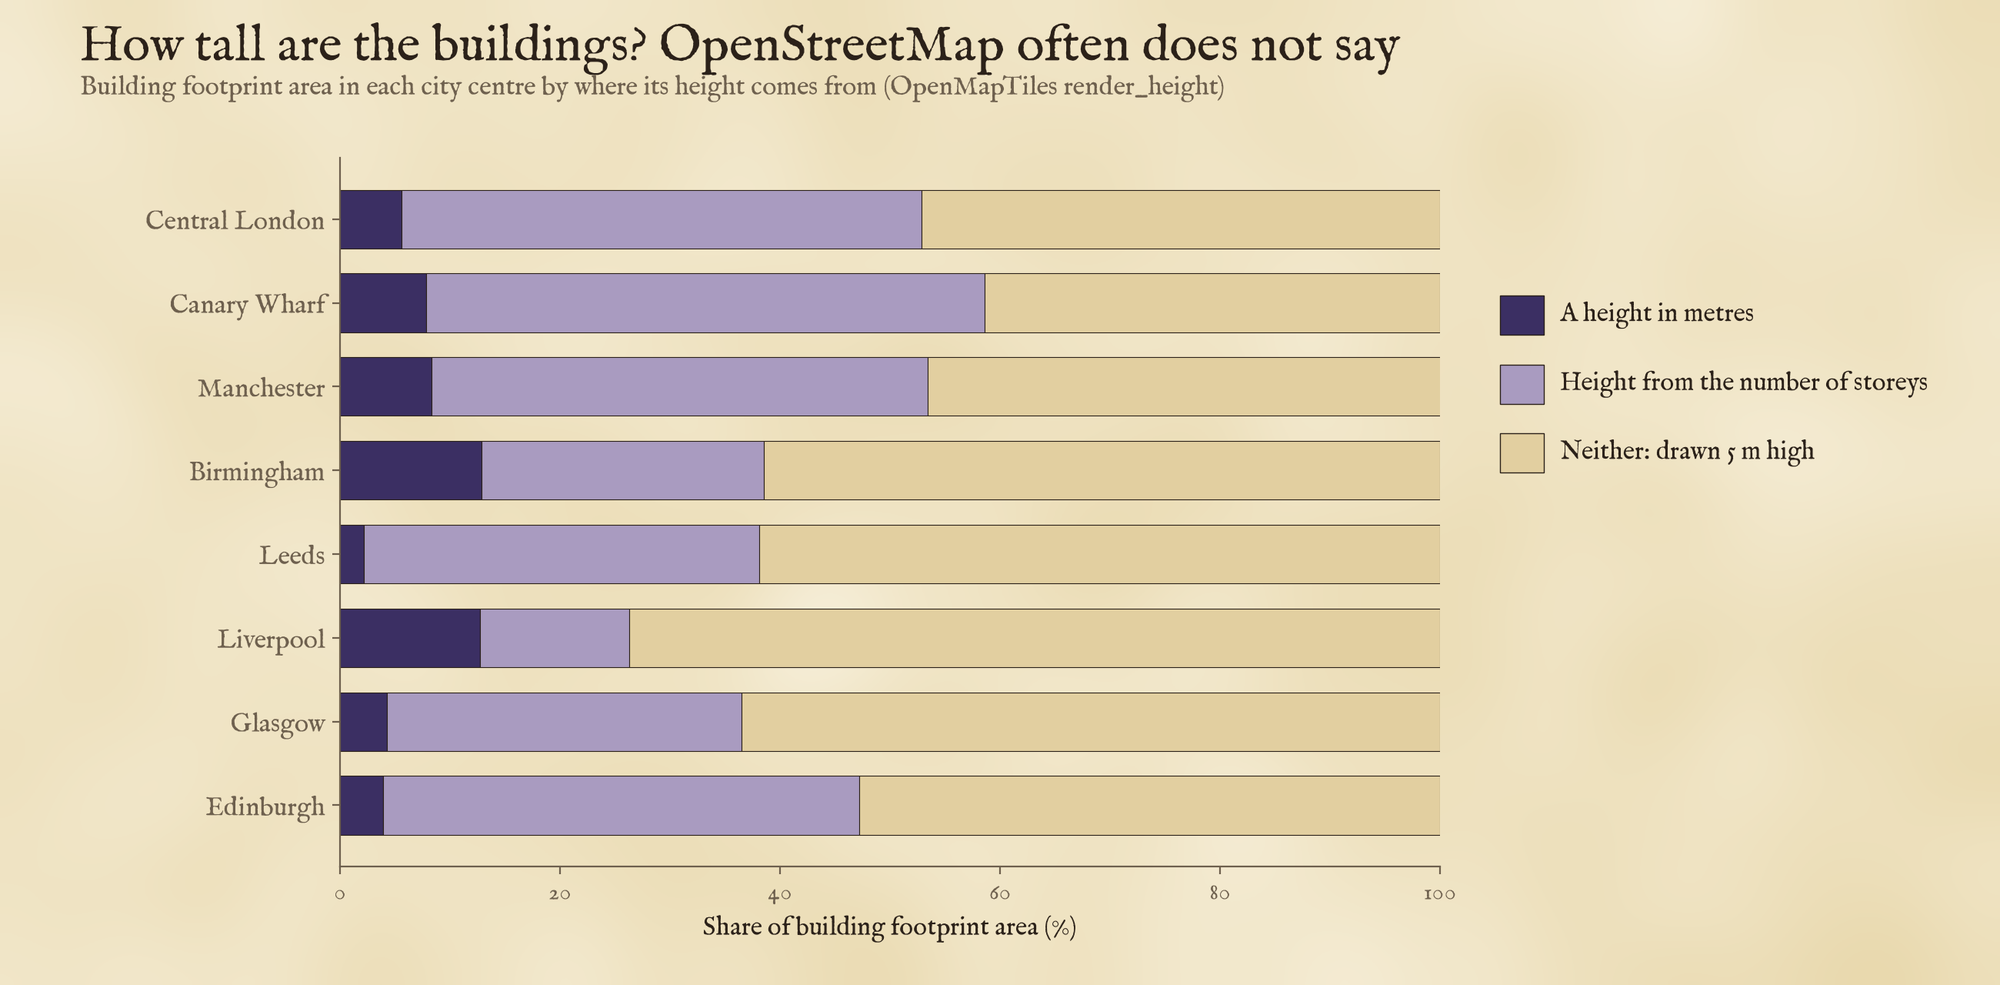
\includegraphics[width=0.9\textwidth]{f_heights.png}
\caption{Where building heights come from, by footprint area.}\label{fig:heights}\end{figure}

\section{Limitations}
Building heights are the main limitation. Between 41.4\% and 73.7\% of building footprint carries the 5 m default; real buildings are usually taller, so the shadows of the ordinary city, and the share of sun it takes, are underestimated. The same bias inflates the towers' share, since some ground counted as shaded only by towers would already be shaded by taller ordinary buildings. Towers nearly always carry a height or a storey count, but heights derived from storeys at 3.66 m each can be too high for residential towers: Landmark Pinnacle at Canary Wharf (233 m, 75 storeys) appears as 275 m ($\lceil 75 \times 3.66 \rceil$) and the tallest tower of South Quay Plaza (215 m, 68 storeys) as 249 m, so the towers' share at Canary Wharf is probably overstated somewhat. The terrain is 90 m and smooths cliffs and cuttings, which matters in Edinburgh. Trees, awnings and bridges are not modelled, raised building parts are treated as solid down to the ground, and the sky is clear. Results are for three days and should not be read as annual sunlight. The tile release is a snapshot of OpenStreetMap and towers under construction may be missing or partial.

\section{Data availability}
The interactive map is at \url{https://maps.tristanhotham.com/tower-shadows/}; data and code at \url{https://github.com/Tristan-Hotham/tower-shadows}. \texttt{cities.csv}, \texttt{streets.csv}, \texttt{open\_spaces.csv} and \texttt{towers.csv} hold the results; \texttt{data/shadows/} the hourly shadow bit planes and hours-of-sun rasters; \texttt{results.json} every number in this paper. Data derived from OpenStreetMap are under the Open Database Licence; text and figures CC BY 4.0; code MIT.

\section*{AI assistance}
I wrote the text, with drafting and editing assistance from Claude (Anthropic), which also helped prepare the analysis code. I reviewed and checked all text and results.

\begin{thebibliography}{9}
\bibitem[Littlefair et al.(2022)]{bre2022} Littlefair, P., King, S., Howlett, G., Ticleanu, C. and Longfield, A. (2022) \textit{Site Layout Planning for Daylight and Sunlight: A Guide to Good Practice} (BR 209), third edition. BRE.
\bibitem[OpenFreeMap(2026)]{openfreemap} OpenFreeMap (2026) Vector tiles of OpenStreetMap in the OpenMapTiles schema. \url{https://openfreemap.org/}
\bibitem[OpenStreetMap(2026)]{osm} OpenStreetMap contributors (2026) OpenStreetMap. Open Database Licence. \url{https://www.openstreetmap.org/}
\bibitem[Saemundsson(1986)]{saemundsson1986} Saemundsson, T. (1986) Atmospheric refraction. \textit{Sky and Telescope} 72, 70.
\bibitem[Spencer(1971)]{spencer1971} Spencer, J. W. (1971) Fourier series representation of the position of the sun. \textit{Search} 2(5), 172.
\end{thebibliography}
\end{document}
